\paragraph{Functional Magnetic Resonance Imaging Data}

Functional Magnetic Resonance Imaging (fMRI) data are typically represented in four dimensions, indicating the measured blood-oxygen-level-dependent (BOLD) signal in temporal sequences $S = \{V_1, ..., V_t\}$ of 3-dimensional volumes $V \in \mathbb{R}^{x \times y \times z}$, each indicating the BOLD signal for all spatial locations of the brain (as defined by three spatial dimensions $x$, $y$, and $z$). A key challenge for the analysis of fMRI data is the high dimensionality and low sample size of its datasets, which typically contain many hundred thousand dimensions (i.e., voxels) for each of several hundred volumes $V$ in each of tens to hundreds of sequences $S$. In this setting, where the number of features exceed the number of samples, standard machine learning approaches are prone to overfitting.

In spite of the low sample size of individual datasets, neuroimaging research can be considered as recently entering a big data era because researchers more frequently share their collected datasets publicly~\citep{markiewicz_2021_openneuro}. The availability of these data open up the opportunity for pre-training in neuroimaging at scale, as recently demonstrated by~\citep{thomas_fmri_2022}, enabling models to utilize the knowledge that can be learned from public functional neuroimaging data for the analysis of individual datasets. Specifically,~\citep{thomas_fmri_2022} evaluate the performance of several self-supervised learning frameworks for functional neuroimaging data by first pre-training models on a broad fMRI dataset spanning $11,980$ fMRI runs from $1,726$ individuals across $34$ datasets and subsequently adapting the pre-trained models to two downstream mental state decoding datasets (namely, the HCP~\citep{van_2013_wu} and MDTB~\citep{king_2019_functional} datasets). In mental state decoding, predictive models are tasked with identifying (i.e., decoding) some set of mental states (e.g., answering questions about a prose story or math problem) from measured brain activity. The authors find that a GPT-based model, pre-trained in a causal learning framework, performs best in decoding the $20$ (HCP) and $26$ (MDTB) mental states of the two downstream datasets.

To evaluate the performance of H3 on fMRI data, we replicate this analysis, using the up- and downstream fMRI datasets that were published by~\citep{thomas_fmri_2022}, treating H3 as a drop-in replacement for the GPT model. To alleviate the high dimensionality challenge of fMRI data, and due to the generally high spatial correlation of brain activity, the original authors have reduced the volumetric time series $S$ to a set $\Theta \in {\theta_1, ..., \theta_n}$ of $n=1,024$ functionally-independent brain networks $\theta$  (as defined by the dictionaries of functional modes (DiFuMo) brain atlas~\citep{dadi_2020_fine}), each describing the BOLD signal for some subset of voxels $v_{x,y,z} \in V$, such that the resulting sequences $X \in \mathbb{R}^{t \times n}$ describe the activity pattern of each brain network $n$ for time points $t$. 

In line with~\citep{thomas_fmri_2022}, we first pre-train models $f(\cdot)$ to predict the distribution of brain activity for the next time point $j$ of an input sequence $X$, using a mean absolute error ($L_{rec}$) training objective given the model's output $\hat{X} \in \mathbb{R}^{t \times n}$: $L_{rec} = \frac{1}{n} \sum_{i=1}^{n} |X_{j,i} - \hat{X}_{j,i}|$; $\hat{X}_{t,n} = b_n + \sum_n f(E^{X})_{t,e} w_{e,n}$; $E^{X}_{t,e} = E^{TR} + E^{pos} + b_e + \sum_n X_{t,n} w_{n,e}$. Here, $E^{TR} \in \mathbb{R}^{e}$ and $E^{pos} \in \mathbb{R}^{e}$ represent learnable embeddings for each possible time point and position of an input sequence (for details, see~\citep{thomas_fmri_2022}). As the sampling frequency of fMRI is variable, the same position of an input sequence can correspond to different time points. Note that $f(\cdot)$ processes the input in a lower-dimensional embedding representation $E^{X} \in \mathbb{R}^{t \times e}$ (with $e=768$ dimensions).

We evaluate two model architectures for $f(\cdot)$, namely, the GPT variant used in ~\citep{thomas_fmri_2022}, with $4$ hidden layers and $12$ attention heads, and a corresponding H3 variant with $4$ hidden layers (with $H=64$ and $m=1$; see section \ref{sec:method}). For both models, the sequence of hidden-states outputs of the last model layer are used to determine $\hat{X}$.

Just as~\citep{thomas_fmri_2022}, we randomly divide the upstream data into distinct training and validation datasets by randomly designating $5\%$ of the fMRI runs of each of the $34$ upstream datasets as validation data (at a minimum of $2$ runs per dataset) and using the rest of the runs for training. During upstream learning, we then randomly sample sequences of $10$ to $100$ time points from the fMRI runs and train models with the ADAM optimizer (with $\beta_1=0.9$, $\beta_2=0.999$, and $\epsilon=1e^{-8}$ ) for $5,000$ steps at a mini-batch size of $512$, and a learning rate of $5e^{-4}$. We apply a linear learning rate decay schedule (with a warm-up phase of 1\% of the total number of training steps), gradient norm clipping at $1.0$, and $L2$-regularisation (weighted by $0.1$). We also apply dropout at a rate of $0.1$ for the GPT-based model (based on~\citep{thomas_fmri_2022}) and evaluate three dropout rates for H3: $0.1$, $0.2$, and $0.3$. 

\begin{figure}[h]
    \centering
    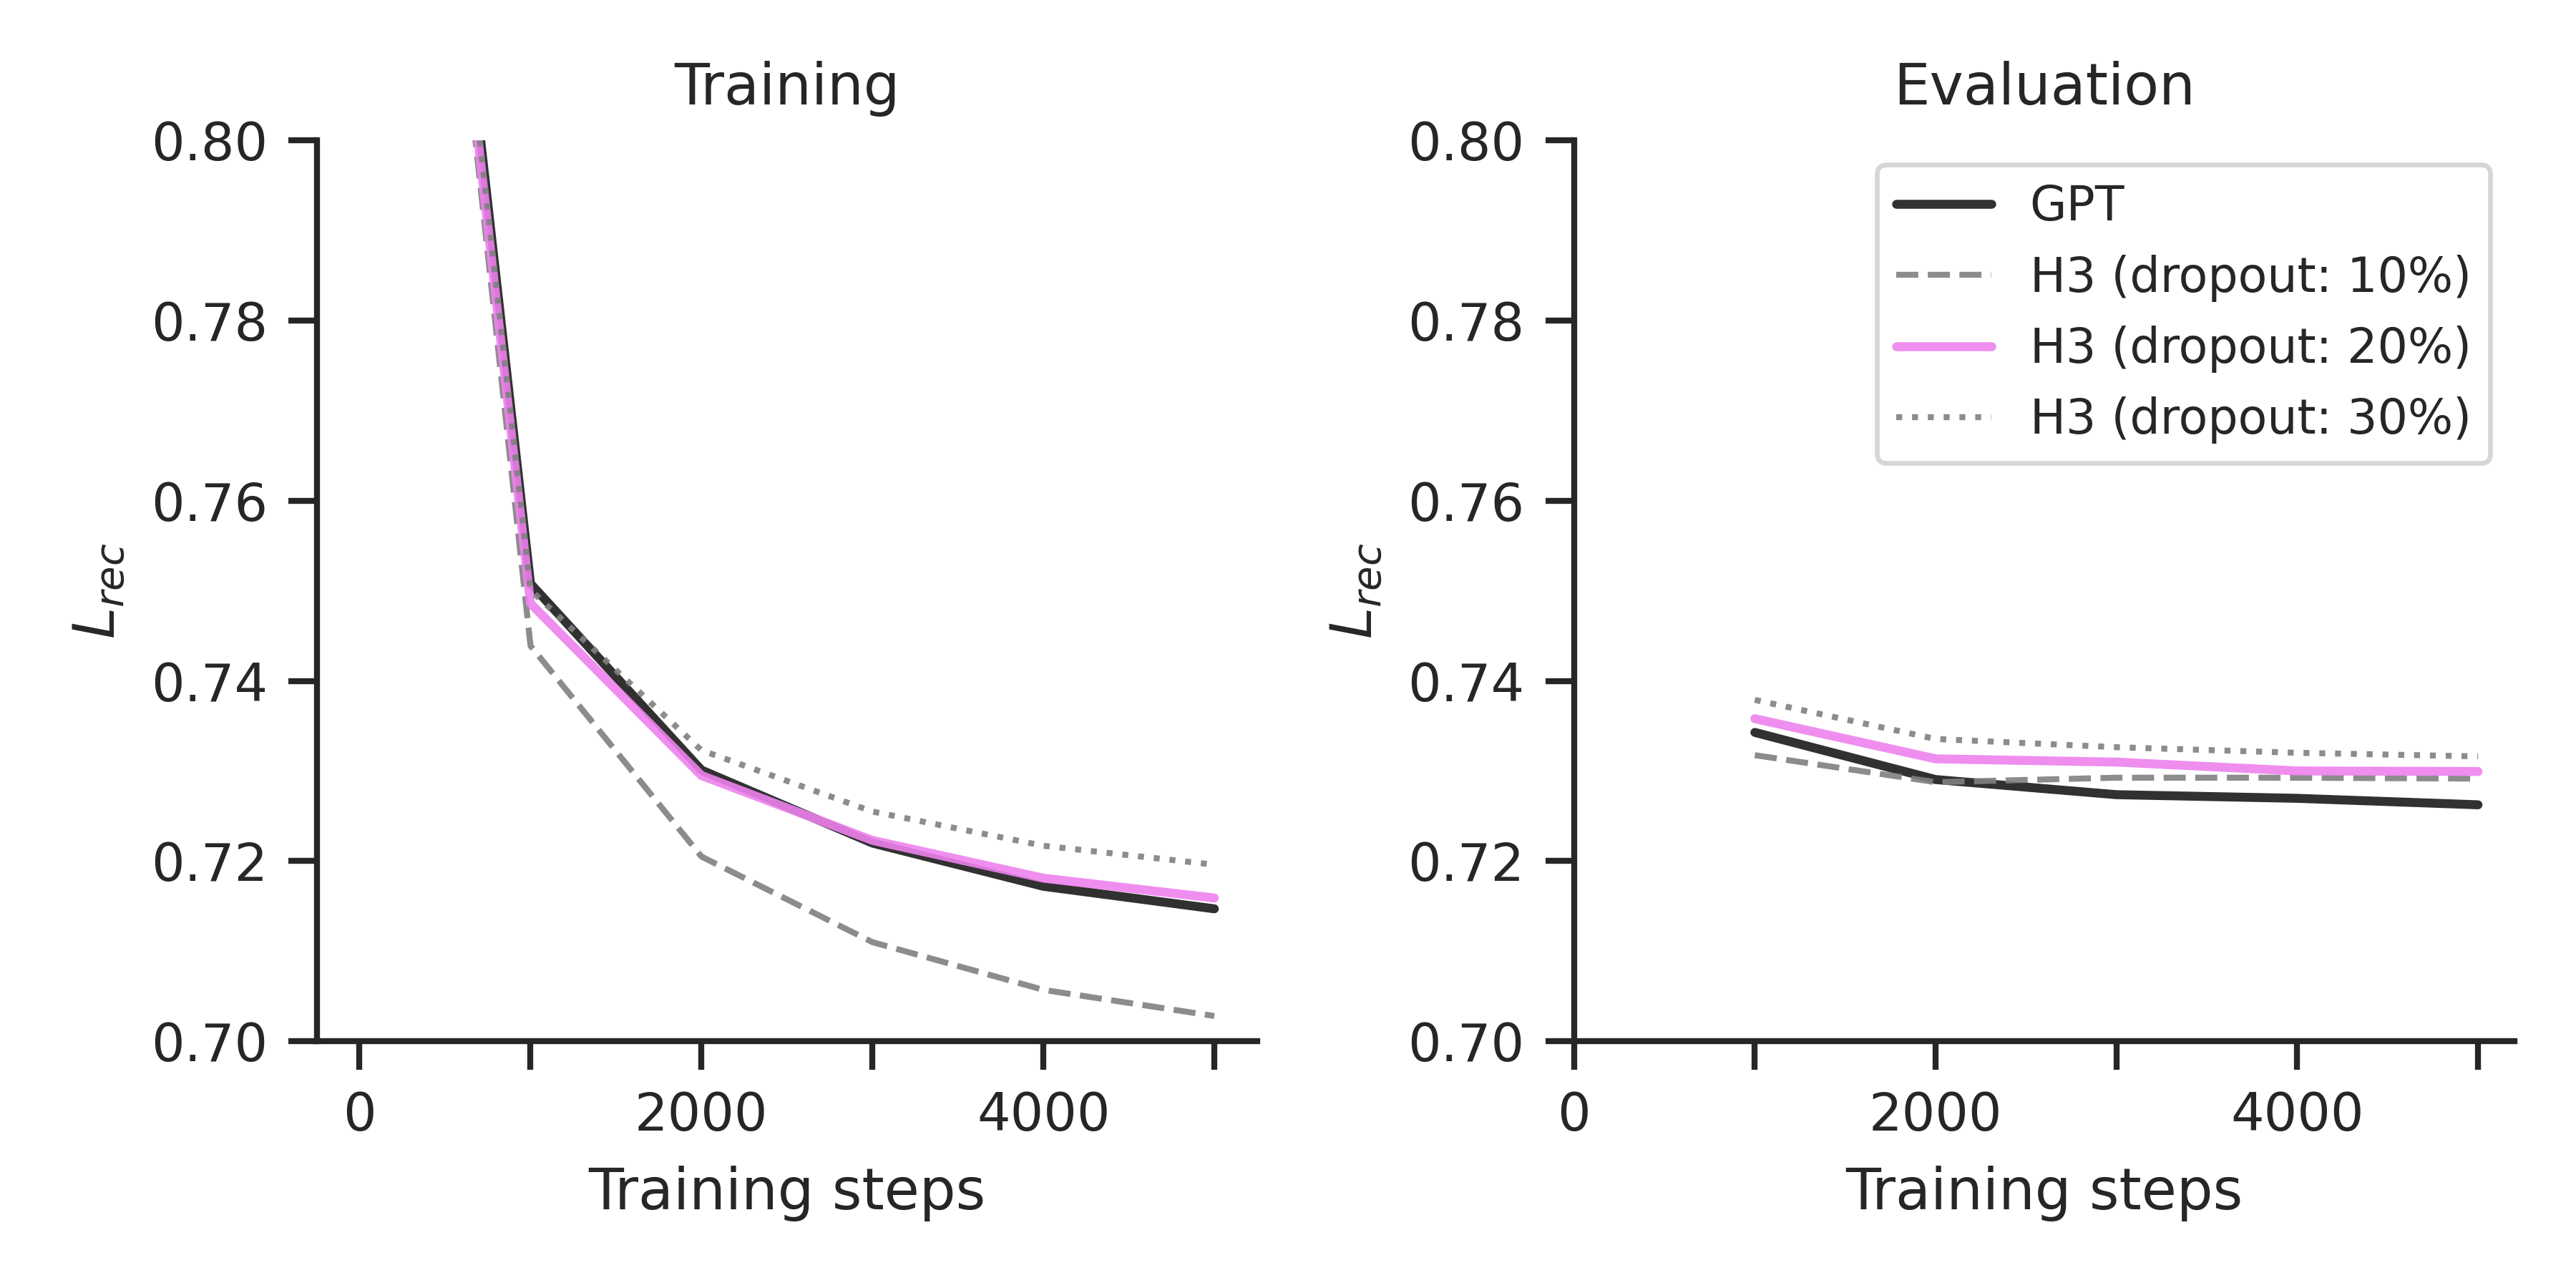
\includegraphics[width=0.65\textwidth]{figs/fmri_upstream-error.png}
    \caption{\label{fig:fmri-upstream} Upstream mean absolute error ($L_{rec}$) in training and evaluation datasets over the course of model training.}
\end{figure}

We find that the H3 variant trained with $0.2$ dropout performs on par with the GPT model, in terms of mean absolute error (Fig.\ \ref{fig:fmri-upstream}), and therefore continue all further analyses with this model variant. We also find that both models exhibit almost identify $L_{rec}$ error distributions throughout the brain, with relatively higher errors in the posterior parietal, occipital, and cingulate cortices as well parts of the limbic system (Fig.\ \ref{fig:fmri-upstream-brain}).

\begin{figure}[h]
    \centering
    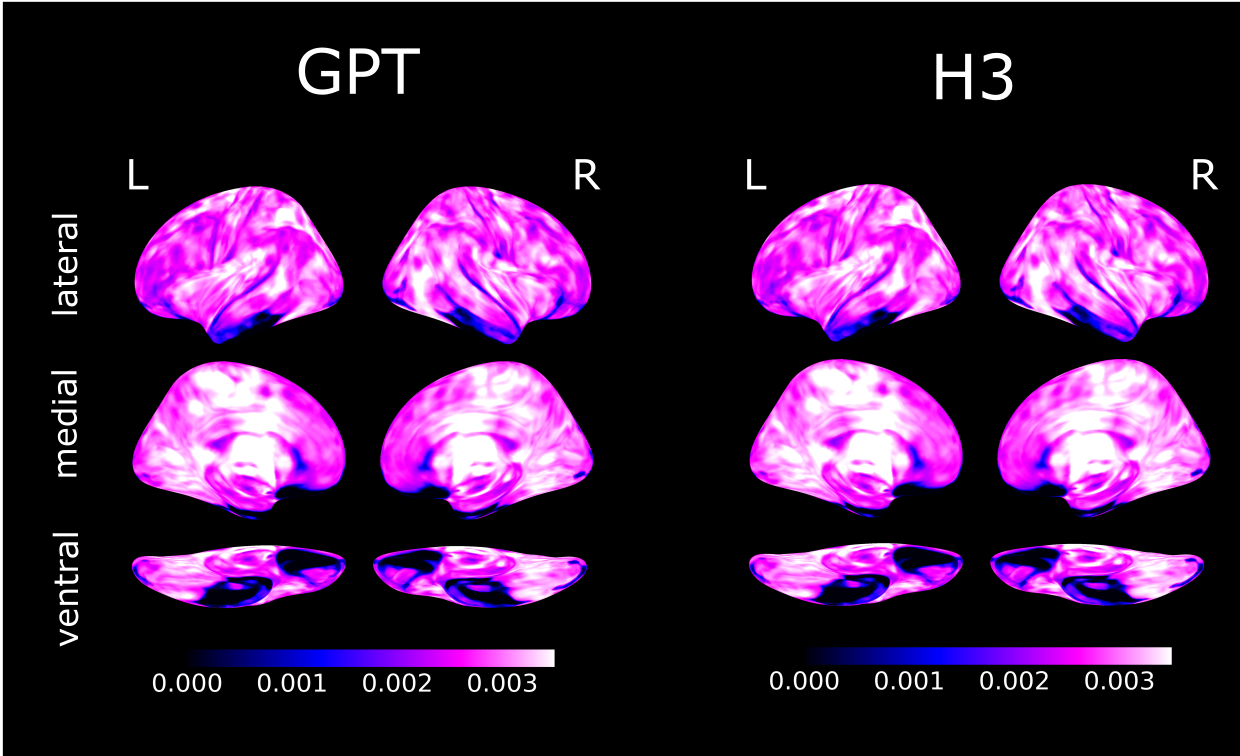
\includegraphics[width=0.5\textwidth]{figs/fmri_upstream-error-brain.png}
    \caption{\label{fig:fmri-upstream-brain} Mean absolute error ($L_{rec}$) of the final pre-trained models for each voxel of the brain projected onto the inflated cortical surface of the FsAverage template~\citep{fischl_2012_freesurfer}.}
\end{figure}

To adapt the pre-trained models to mental state decoding, we add a learnable classification embedding $E^{cls} \in \mathbb{R}^{n}$ to the end of input sequences $X$ and forward the model's prediction $f(E^{X})$ to a decoding head $p(\cdot)$, composed of a dense hidden layer with $e$ model units (one for each embedding dimension, with $tanh$ activation) as well as a $softmax$ output layer with one model unit $i$ for each considered mental state in the data. Accordingly, we adapt models by optimizing a standard cross entropy loss objective: $L_{cls} = - \sum_i y_i \log \ {p(f(E^X))_i}$, where $y_i$ indicates a binary variable that is $1$ if $i$ is the correct mental state and $0$ otherwise.

During downstream adaptation, we begin training with the respective pre-trained model parameters and then allow all parameters to change freely. Similar to~\citep{thomas_fmri_2022}, we randomly split each of the two downstream datasets into distinct training and test datasets, each comprising $40$ (HCP) or $10$ (MDTB) distinct individuals. We adapt models for $750$ steps at a mini-batch size of $256$ and a learning rate of $5e^{-5}$ (otherwise using the same learning parameters as for upstream training). Importantly, we repeat each downstream training run $20$ times using different random seeds, leading to different random splits of the data and variability in other non-deterministic training factors (such as random initialization and data shuffling).

As for the upstream data, the H3 and GPT-based models generally perform on par in their mental state decoding performances in the two left-out test datasets (Table \ref{table:fmri-downstream}).

\begin{table}[h]
    % \captionsetup{font=small}
    \small
    \centering
    %\vspace{-1em}
    \caption{\label{table:fmri-downstream} Downstream adaptation performance of models pre-trained on fMRI data, averaged over $20$ training runs with varying random seeds. F1-scores are macro-averaged.}
    %   \vspace{1em}
    {
        \begin{tabular}{@{}|c|c|cc|@{}}
        %   \specialrule{.15em}{.05em}{.05em}
        \hline
        Dataset & Model & Acc. ($\pm 95\% \text{CI}$) & F1 ($\pm 95\% \text{CI}$)\\ % & Training time \\
        %   \specialrule{.15em}{.05em}{.05em}
        \hline
        HCP & GPT & $88.44$ ($\pm 0.39$) & $87.24$ ($\pm 0.39$) \\
         & H3 & $88.75$ ($\pm 0.33$) & $87.16$ ($\pm 0.37$) \\ \hline
        MDTB & GPT & $89.47$ ($\pm 0.44$) & $88.74$ ($\pm 0.54$) \\
         & H3 & $88.25$ ($\pm 0.45$) & $85.76$ ($\pm 0.61$) \\ \hline
        \end{tabular}
    }
    %\vspace{-1em}
\end{table}